%! alt An oblique view of the cube whose corners have coordinates 0 and 2, with the nine points of its bottom face marked. A triangle PQR with vertices P = (2, 0, 1), Q = (0, 1, 2) and R = (2, 2, 2) is drawn above its shaded shadow P'Q'R' on the bottom face z = 0, and dashed vertical segments join each vertex to its shadow.
%! after_paragraph 1
%! scale 12/5
% The shared preamble of every Cevian figure. pipeline/figures turns these colours into theme-aware paint,
% and refuses any other colour, so draw only with them:
%   figink (lines and labels), figaux (construction lines), figaccent (the object the argument turns on),
%   figtint and figaccenttint (light fills).
\documentclass[border=1.5pt]{standalone}
\usepackage{tkz-euclide}
\definecolor{figink}{RGB}{0,0,0}
\definecolor{figaux}{RGB}{85,85,85}
\definecolor{figaccent}{RGB}{192,57,43}
\definecolor{figtint}{RGB}{221,221,221}
\definecolor{figaccenttint}{RGB}{245,213,208}
% tkz-euclide's defaults draw circles, compasses and marks in 50% grey and fill points with a tint.
\makeatletter
\def\tkz@otherlinecolor{figink}
\def\tkz@euc@circlecolor{figink}
\def\tkz@euc@compasscolor{figink}
\def\tkz@euc@mkcolor{figink}
\def\tkz@mk@fill{figink}
\def\tkz@euc@pointfillcolor{figink}
\makeatother
\tkzSetUpLine[color=figink,line width=.7pt]
\tkzSetUpArc[color=figink,line width=.7pt]
\tkzSetUpCompass[color=figink,line width=.5pt]
\tkzSetUpPoint[color=figink,fill=figink,size=3.1pt]
\tikzset{
  every picture/.style={line cap=round,line join=round,color=figink},
  circle style/.append style={color=figink,line width=.7pt},
  aux/.style={color=figaux,line width=.45pt,dash pattern=on 2.6pt off 2pt},
  key/.style={color=figaccent,line width=1pt},
  mk/.style={color=figink,line width=.5pt},
  lbl/.style={color=figink,inner sep=2.2pt},
  len/.style={color=figink,inner sep=1.5pt,font=\small},
}

\begin{document}
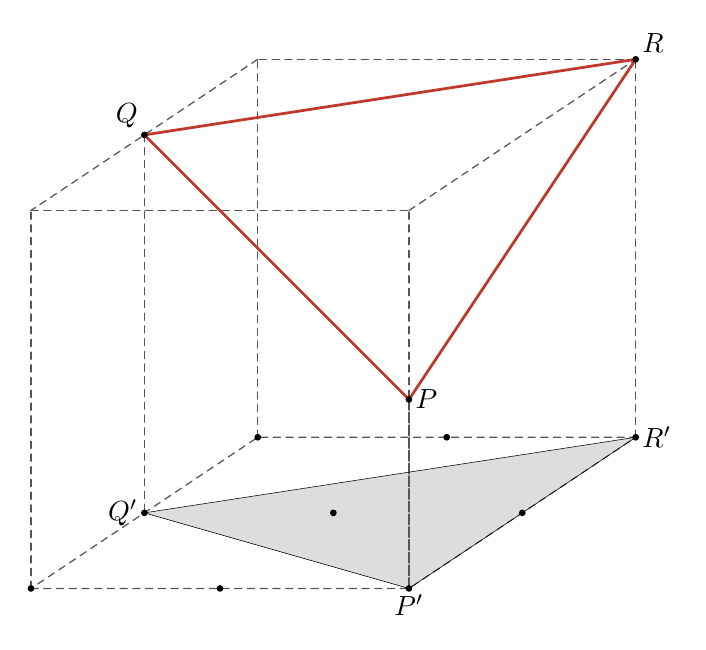
\begin{tikzpicture}
\tkzDefPoint(0.0,0.0){O} %! O = (0, 0)
\tkzDefPoint(4.8000000,0.0){X} %! X = (2, 0)
\tkzDefPoint(2.8800000,1.9200000){Y} %! Y = (6/5, 4/5)
\tkzDefPoint(7.6800000,1.9200000){W} %! W = (16/5, 4/5)
\tkzDefPoint(0.0,4.8000000){Z} %! Z = (0, 2)
\tkzDefPoint(4.8000000,4.8000000){XZ} %! XZ = (2, 2)
\tkzDefPoint(2.8800000,6.7200000){YZ} %! YZ = (6/5, 14/5)
\tkzDefPoint(7.6800000,6.7200000){WZ} %! WZ = (16/5, 14/5)
\tkzDefPoint(2.4000000,0.0){G} %! G = (1, 0)
\tkzDefPoint(1.4400000,0.96000000){H} %! H = (3/5, 2/5)
\tkzDefPoint(3.8400000,0.96000000){J} %! J = (8/5, 2/5)
\tkzDefPoint(6.2400000,0.96000000){K} %! K = (13/5, 2/5)
\tkzDefPoint(5.2800000,1.9200000){L} %! L = (11/5, 4/5)
\tkzDefPoint(4.8000000,2.4000000){P} %! P = (2, 1)
\tkzDefPoint(1.4400000,5.7600000){Q} %! Q = (3/5, 12/5)
\tkzDefPoint(7.6800000,6.7200000){R} %! R = (16/5, 14/5)
\tkzDefPoint(4.8000000,0.0){Pp} %! Pp = (2, 0)
\tkzDefPoint(1.4400000,0.96000000){Qp} %! Qp = (3/5, 2/5)
\tkzDefPoint(7.6800000,1.9200000){Rp} %! Rp = (16/5, 4/5)
%! fact parallel(P, Pp, Q, Qp)
%! fact parallel(Q, Qp, R, Rp)
%! fact parallel(P, Pp, O, Z)
%! fact parallel(O, X, Y, W)
%! fact parallel(O, Y, X, W)
%! fact midpoint(J, H, K)
%! fact midpoint(G, O, X)
\tkzFillPolygon[color=figtint](Pp,Qp,Rp)
\tkzDrawPolygon[aux](O,X,W,Y)
\tkzDrawSegment[aux](Z,XZ)
\tkzDrawSegment[aux](XZ,WZ)
\tkzDrawSegment[aux](WZ,YZ)
\tkzDrawSegment[aux](YZ,Z)
\tkzDrawSegment[aux](O,Z)
\tkzDrawSegment[aux](X,XZ)
\tkzDrawSegment[aux](W,WZ)
\tkzDrawSegment[aux](Y,YZ)
\tkzDrawSegment[aux](P,Pp)
\tkzDrawSegment[aux](Q,Qp)
\tkzDrawPolygon(Pp,Qp,Rp)
\tkzDrawPolygon[key](P,Q,R)
\tkzDrawPoints(O,X,Y,W,G,H,J,K,L,P,Q,R)
\tkzLabelPoint[right,lbl](P){$P$}
\tkzLabelPoint[above left,lbl](Q){$Q$}
\tkzLabelPoint[above right,lbl](R){$R$}
\tkzLabelPoint[below,lbl](Pp){$P'$}
\tkzLabelPoint[left,lbl](Qp){$Q'$}
\tkzLabelPoint[right,lbl](Rp){$R'$}
\end{tikzpicture}
\end{document}
